\documentclass{article}
\usepackage{amsmath}
\usepackage[mathletters]{ucs}
\usepackage[utf8x]{inputenc}
\usepackage[margin=1.5in]{geometry}
\usepackage{enumerate}
\newtheorem{theorem}{Theorem}
\usepackage[dvipsnames]{xcolor}
\usepackage{pgfplots}
\setlength{\parindent}{0cm}
\usepackage{graphics}
\usepackage{graphicx} % Required for including images
\usepackage{subcaption}
\usepackage{bigintcalc}
\usepackage{pythonhighlight} %for pythonkode \begin{python}   \end{python}
\usepackage{appendix}
\usepackage{arydshln}
\usepackage{physics}
\usepackage{tikz-cd}
\usepackage{booktabs} 
\usepackage{adjustbox}
\usepackage{mdframed}
\usepackage{relsize}
\usepackage{physics}
\usepackage[thinc]{esdiff}
\usepackage{fixltx2e}
\usepackage{esint}  %for lukket-linje-integral
\usepackage{xfrac} %for sfrac
\usepackage{hyperref} %for linker, må ha med hypersetup
\usepackage[noabbrev, nameinlink]{cleveref} % to be loaded after hyperref
\usepackage{amssymb} %\mathbb{R} for reelle tall, \mathcal{B} for "matte"-font
\usepackage{listings} %for kode/lstlisting
\usepackage{verbatim}
\usepackage{graphicx,wrapfig,lipsum,caption} %for wrapping av bilder
\usepackage{mathtools} %for \abs{x}
\usepackage[norsk]{babel}
\definecolor{codegreen}{rgb}{0,0.6,0}
\definecolor{codegray}{rgb}{0.5,0.5,0.5}
\definecolor{codepurple}{rgb}{0.58,0,0.82}
\definecolor{backcolour}{rgb}{0.95,0.95,0.92}
\pagecolor[rgb]{0.075,0.075,0.075} \color[rgb]{1,1,1} %TODO: Slett når ferdig%
\lstdefinestyle{mystyle}{
    backgroundcolor=\color{backcolour},   
    commentstyle=\color{codegreen},
    keywordstyle=\color{magenta},
    numberstyle=\tiny\color{codegray},
    stringstyle=\color{codepurple},
    basicstyle=\ttfamily\footnotesize,
    breakatwhitespace=false,         
    breaklines=true,                 
    captionpos=b,                    
    keepspaces=true,                 
    numbers=left,                    
    numbersep=5pt,                  
    showspaces=false,                
    showstringspaces=false,
    showtabs=false,                  
    tabsize=2
}

\lstset{style=mystyle}
\author{Oskar Idland}
\title{FYS2140 - Oblig 4}
\date{}
\begin{document}
\maketitle
\newpage

\section*{\underline{A Diskusjonsoppgaver}}
\subsection*{Oppgave 1}
Det er flere av svarene som er delvis korrekte. 
\begin{enumerate}[\bf A:]
    \item Ser strengt tatt ikke veldig fysisk ut, men vi kan selvsagt tolke grafen for å hente ut informasjon vi kan bruke i den virkelige verden. 
    \item Kvantemekanikken er akkurat hva vi trenger for å tolke en denne type bølgefunksjon. 
    \item Bølgefunksjonen \textit{kan} beskrive en stor partikkel, men det er informasjon vi ikke har. 
    \item Bølgefunksjonen \textit{kan} beskrive en liten partikkel, men det er informasjon vi ikke har. 
    \item Siste alternativ er hva jeg tolker som det mest korrekte svaret. Bølgefunksjonen viser oss at det er mest sannsynlig å finne en partikkel ved $x = 50$
\end{enumerate}
\subsection*{Oppgave 2}
\begin{enumerate}[a)]
    \item Bølgefunksjonen $Ψ$ er en kompleks funksjon som beskriver en partikkels kvantemekaniske tilstander som posisjon, bevegelsesmengde, tid og spin. Ettersom funksjonen er kompleks vil dens amplitude ikke ha noe direkte fysisk tolkning. 
    
    Den reelle funksjonen $\left|Ψ\right|^2 $ er kvadratet av bølgefunksjonen. Denne funksjonen er alltid et positivt tall, og beskriver sannsynligheten for å finne en partikkel i et punkt, eller område hvis integrert, til en hver tid. 
    
    $x(t)$ er en klassisk funksjon som beskriver nøyaktig posisjonen til en hver tid. 
    \item Via $Ψ$ kan vi få informasjon om hvilke kvantemekaniske tilstander det den beskriver vil ha samt hvor sannsynlig det er å finne en partikkel i et punkt eller områder. 
    
    Via $x(t)$ kan vi få informasjon om nøyaktig posisjonen til en partikkel til en hver tid.
\end{enumerate}
\subsection*{Oppgave 3}
\begin{enumerate}[\bf A:]
    \item Forventningsverdien til $\left<x\right>$ er bare den gjennomsnittsverdien vi måler over en stor mengde målinger. Det er ikke gitt at det er en mulig mulig verdi for posisjon. Hvis $\left<x\right>$ er en mulig verdi, vil hvis det også være den mest sannsynlige. 
    \item Sannsynligheten for å måle forventningsverdien, kan være null. Dette er ikke uvanlig når mulig verdier er diskrete. 
    \item Det stemmer at $\left<x\right>$ er gjennomsnittet vi hadde målt over en stor mengde målinger.
\end{enumerate}
\section*{\underline{B Regneoppgaver}}
\subsection*{Oppgave 4}
\begin{enumerate}[a)]
    \item For å normalisere $Ψ$ må vi løse $\int_{-\infty}^{\infty} \left|Ψ\right|^2 dx = 1$. 
    \[
    \left|Ψ\right|^2 = Ψ ⋅  Ψ^{*} = Ae^{-λ \left|x\right| }e^{-iωt} ⋅ Ae^{-λ \left|x\right| }e^{iωt} = A^2e^{-2λ \left|x\right| }
    \]
    \[
    ∫_{-∞}^{∞} A^2e^{-2λ\left|x\right|} \ \mathrm{d}x = 1 ⇒ A^2 ∫_{-∞}^{∞} e^{-2λ\left|x\right|} \ \mathrm{d}x = 1
    \]
    \[
    A^2 \left(\underbrace{∫_{-∞}^{0} e^{2λx} \ \mathrm{d}x}_{\frac{1}{2λ}} + \underbrace{∫_{0}^{∞} e^{-2λx}\ \mathrm{d}x}_{\frac{1}{2λ}} \right) = 1
    \]
    \[
    A^2 \frac{1}{λ} = 1 ⇒ A = \sqrt{λ}
    \]
    \item Forventningsverdien til $x$ finner vi ved å bruke den normaliserte bølgefunksjonen.
    \[
    \left<x\right> = ∫_{-∞}^{∞} Ψ^{*}xΨ \ \mathrm{d}x = \int_{-\infty}^{\infty} λxe^{-2λ\left|x\right|} \ \mathrm{d}x
    \]
    Ettersom en funksjonen er symmetrisk om $x = 0$, men med motsatt fortegn vil integralet bli lik null. Da følger det at 
    \[
    \underline{\underline{\left<x\right> = 0.}}
    \]
    Forventningsverdien til $x^2$ er gitt ved 
    \[
    \left<x^2\right> = ∫_{-∞}^{∞} Ψ^{*}x^2Ψ \ \mathrm{d}x = \int_{-\infty}^{\infty} λx^2e^{-2λ\left|x\right|} \ \mathrm{d}x. 
    \]
    Ettersom funksjonen er symmetrisk om $x=0$ vil integralet bli likt på begge sider. Vi tar for oss det positive intervallet for $0\le x\le ∞$, og ganger med to. 
    \[
    2λ∫_{0}^{∞} x^2e^{-2λx} \ \mathrm{d}x = \frac{1}{2λ^2}
    \]
    \[
    \underline{\underline{\left<x^2\right> = \frac{1}{2λ^2}}}
    \]
    \item Vi finner standardavviket $σ$ på følgende måte.
    \[
    σ = \sqrt{\left<x^2\right> - \left<x\right>^2} = \sqrt{\frac{1}{2λ^2} - 0^2} = \frac{1}{\sqrt{2}λ}
    \]
    \begin{figure}[h!]
      \centering
      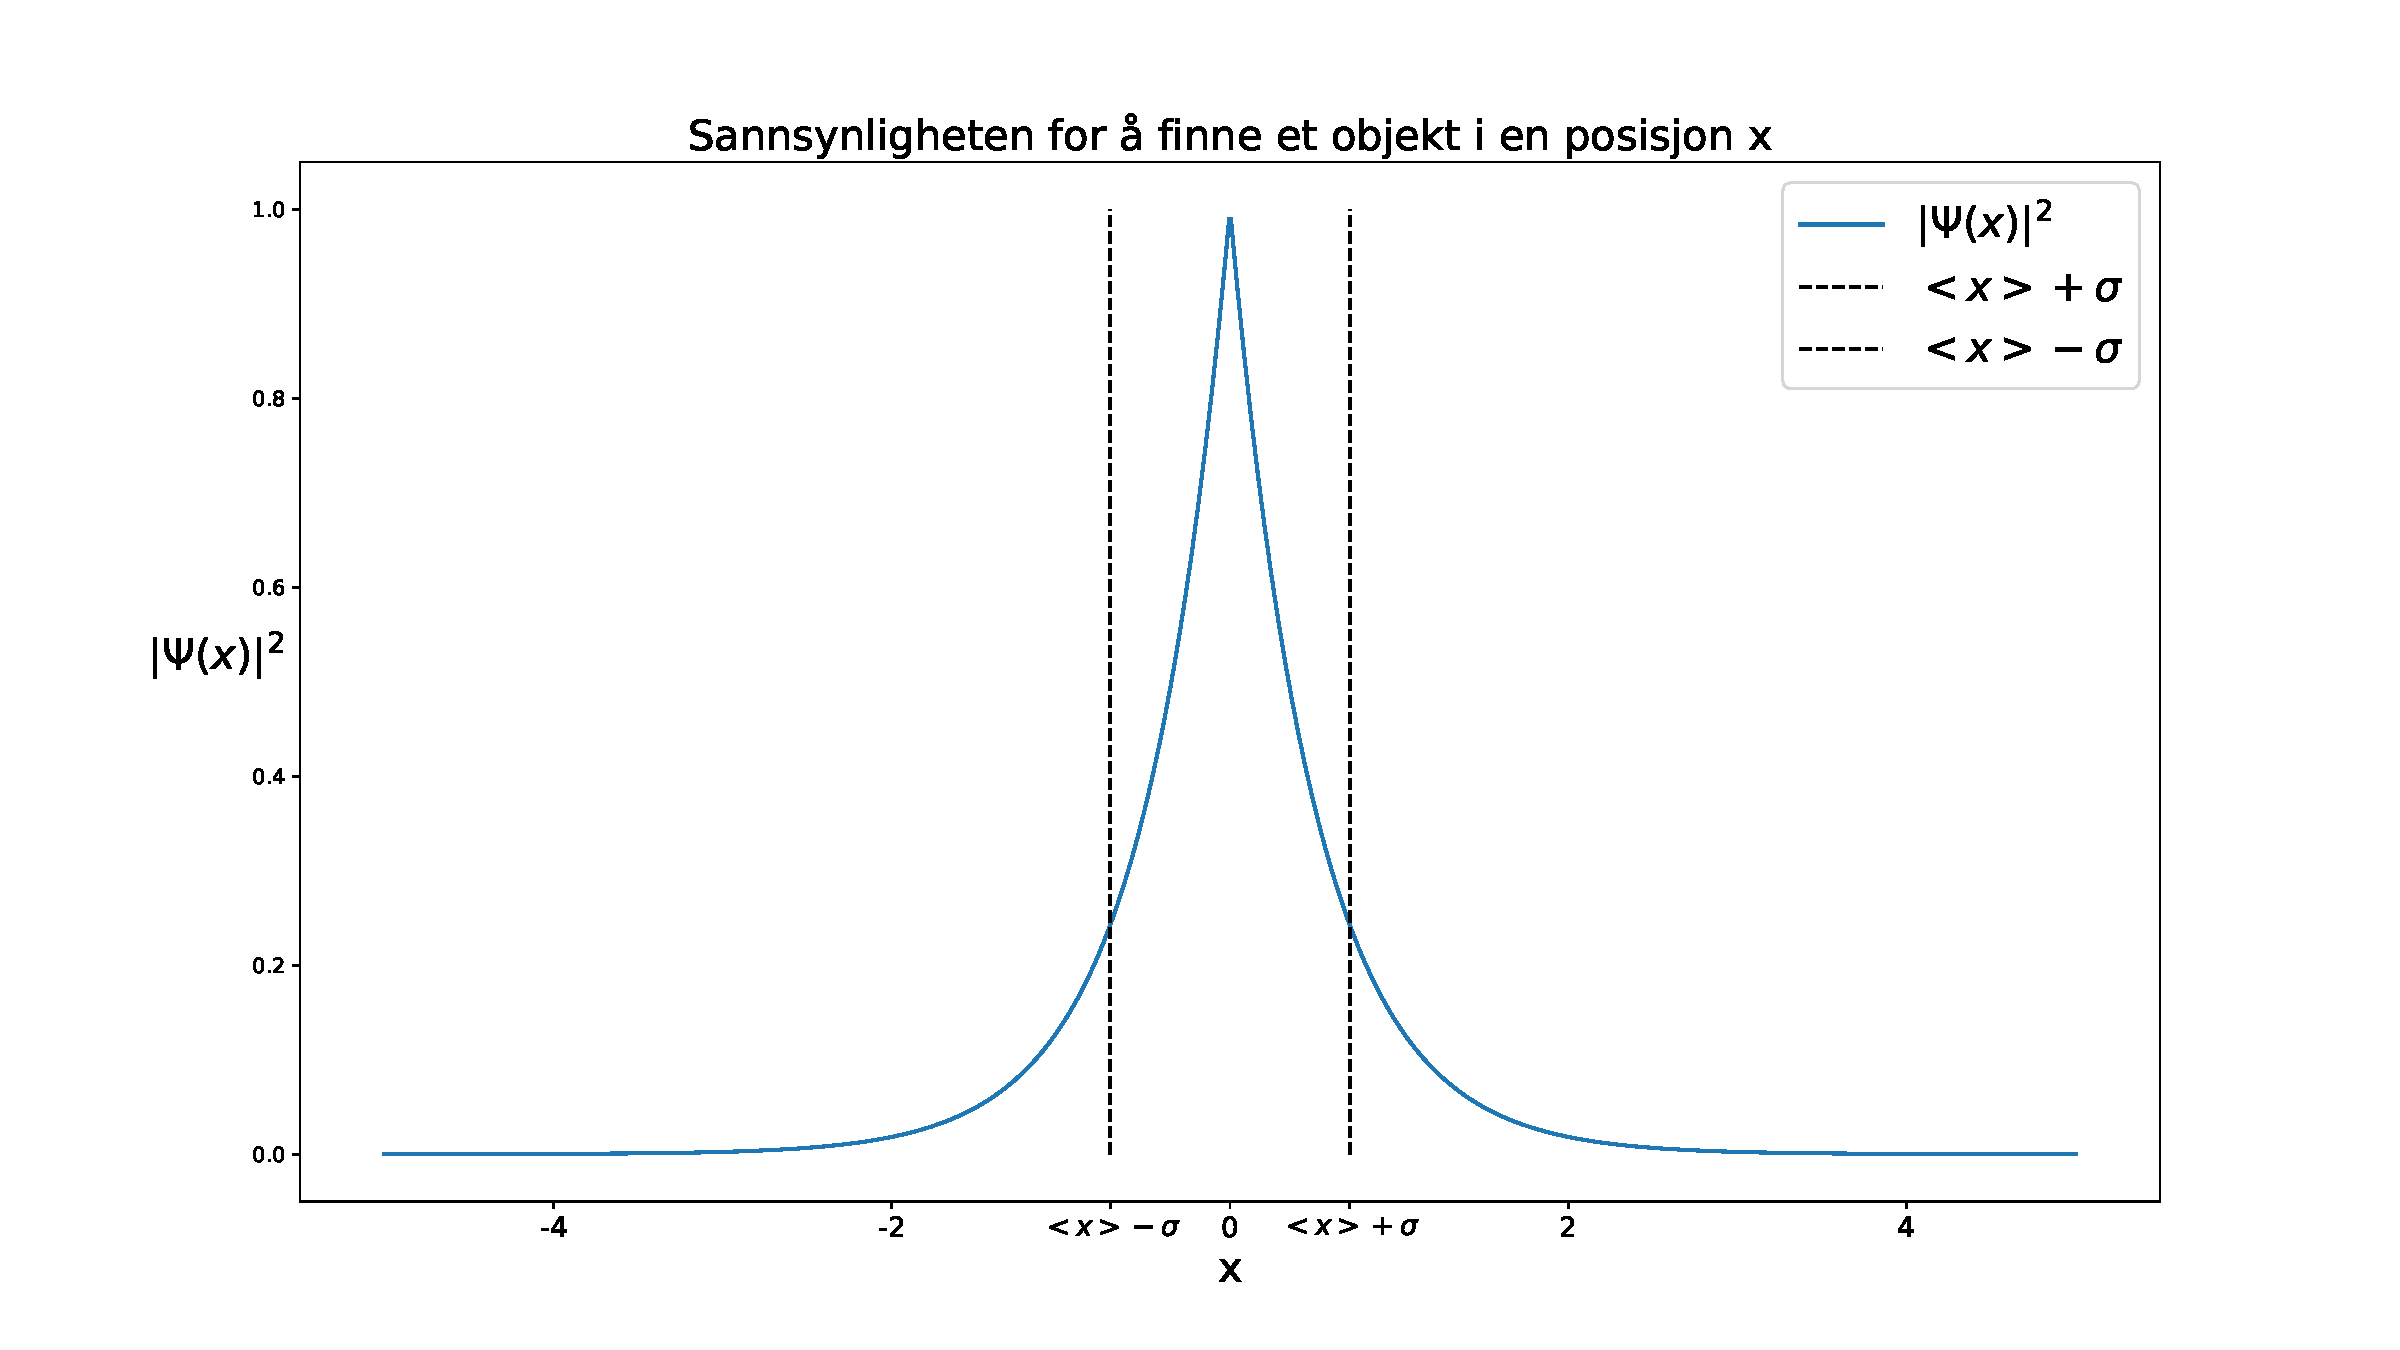
\includegraphics[width = \textwidth]{4.c.pdf}
      \caption{Oppgave 4.c}
      \label{fig: 4.c}
    \end{figure}
    \item Vi finner sannsynligheten for å finne en partikkel utenfor et område ved å bruke 68-95-99.7 regelen. Ettersom partikkelen er i intervallet $x_2\le x\le x_1$ som er i intervallet $-σ\le x \le σ$, vet vi at det er 68.3 \% sannsynlighet for at partikkelen befinner seg i dette området. Da er det 100\% - 68.3\% = 31.7\% sannsynlighet for at partikkelen befinner seg utenfor dette området. 
\end{enumerate}

\subsection*{Oppgave 5}
\begin{enumerate}[a)]
    \item Vi finner $A$ på samme måte som i oppgave 4. Ettersom funksjonen er symmetrisk om $x=0$ vil integralet bli likt på begge sider. Vi tar for oss det positive intervallet for $0\le x\le ∞$, og ganger med to.
    \[
    ∫_{-∞}^{∞} \left|Ψ\right|^2 \ \mathrm{d}x = 1 ⇒ ∫_{-∞}^{∞} Ψ^{*}Ψ \ \mathrm{d}x = 1
    \]
    \[
    ∫_{-∞}^{∞} A^2 e^{-a(mx^2 / ℏ+it)} ⋅ e^{-a(mx^2 / ℏ - it)} \ \mathrm{d}x = 1
    \]
    \[
    ∫_{-∞}^{∞} A^2e^{-2a(mx^{2} / ℏ)} \ \mathrm{d}x
    \]
    Vi ser i Rottmann (2019 s, 155 nr. 49) at 
    \[
    ∫_{-∞}^{∞} e^{-λx^2} \ \mathrm{d}x = \sqrt{\frac{π}{λ}}
    \]
    Hvis vi substituerer inn $\displaystyle λ = \frac{2am}{ℏ}$ i dette uttrykket får vi følgende. 
    \[
    A^2 \sqrt{\frac{πℏ}{2am}} = 1 ⇒ A^2 \sqrt{\frac{h}{4am}} = 1 ⇒ A = \sqrt[4]{\frac{4am}{h}}
    \]
    \item 
    Vi finner potensialet ved å løse Schrödingerligningen for $V$
    \[
    V(x) = Ψ^{-1} \left(iℏ\frac{∂ Ψ}{∂ t} + \frac{ℏ^2}{2m}\frac{∂^2 Ψ}{∂ x^2}\right)    
    \]
    \[
    Ψ^{-1} = A^{-1}e^{a(mx^2 / ℏ + it)}
    \]
    \[
    iℏ\frac{∂ Ψ}{∂ t} = iℏA\left(-ie^{-a(mx^2 /ℏ + it)}\right) = A ℏe^{-a(mx^2 / ℏ + it)}
    \]
    \[
    \frac{ℏ^2}{2m} \frac{∂^2 Ψ}{∂ x^2} = \frac{ℏ^2}{2m}A \left(-2amx / ℏ\right)^2e^{-a(mx^2 /ℏ + it)} = 2Ama^2x^2e^{-a(mx^2 /ℏ + it)} 
    \]
    \[
    V(x) = A^{-1}e^{a(mx^{2} / ℏ + it)} \left(Aℏe^{-a(mx^2 /ℏ + it)}+ 2Ama^2x^2e^{-a(mx^2 / ℏ + it)}\right)
    \]
    \[
    V(x) = 2ma^2x^2 ℏ
    \]
    \item 
    Vi finner forventningsverdien $\left<x\right>$ ved samme metode som i oppgave 4.
    \[
    \left<x\right> = ∫_{-∞}^{∞} Ψ^{*}xΨ \ \mathrm{d}x
    \]
    Vi kan se at funksjonen er symmetrisk om $x=0$ og at funksjonen $x$ er symmetrisk, men med motsatt fortegn om $x=0$. Derfor vil integralet av produktene deres bli null. Da vet vi at 
    \[
    \underline{\underline{\left<x\right> = 0}}
    \]
    Vi finner forventningsverdien $\left<x^2\right>$ ved samme metode som i oppgave 4. Her ser vi at begge funksjoner er symmetriske om $x=0$, så vi kan ta integralet fra $0$ til $∞$ og gange med to.
    \[
    \left<x^2\right> = 2∫_{0}^{∞} Ψ^{*}x^2Ψ \ \mathrm{d}x = 2∫_{0}^{∞} x^2A^2e^{-2a(mx^2 / ℏ)} \ \mathrm{d}x
    \]
    Vi ser i Rottmann (2019 s, 155 nr. 50) at
    \[
    ∫_{0}^{∞} e^{-λx^2}x^{k} \ \mathrm{d}x = \frac{1}{2}λ^{-\frac{k+1}{2}} \underbrace{Γ\left(\frac{k+1}{2}\right)}_{\left(\frac{k+1}{2} - 1\right)!}
    \]
    Vi setter inn $\displaystyle λ = \frac{2am}{ℏ}$ og $k=2$ i dette uttrykket og får følgende.
    \[
    \sqrt{\frac{4am}{ℏ}} \left(\frac{2am}{ℏ}\right)^{- \frac{3}{2}} \underbrace{Γ\left(\frac{3}{2}\right)}_{\frac{1}{2}! = \frac{\sqrt{π}}{2}}
    \]
    \[
    \left<x^2\right> = \sqrt{\frac{4am}{ℏ}}\left(\frac{2am}{ℏ}\right)^{- 3 / 2} \frac{1}{2} \sqrt{π} = \underline{\underline{\sqrt{\frac{amπ}{ℏ}\left(\frac{2am}{ℏ}\right)^{-3}}}}
    \]
    \colorbox{red}{Alt her er feil. Ikke hvordan man finner forventet bevegelsesmengde}
    For å finne forventningsverdien til bevegelsesmengden $p$ må vi løse følgende 
    \[
    \left<p\right> = ∫_{-∞}^{∞} Ψ^{*}pΨ \ \mathrm{d}x = p ∫_{-∞}^{∞} e^{-2a(mx^2 / ℏ)} \ \mathrm{d}x
    \]
    Integralet er symmetrisk om $x=0$ så vi kan ta integralet fra $0$ til $∞$ og gange med to. Vi ser igjen i Rottmann (2019 s, 155 nr. 49) at
    \[
    ∫_{0}^{∞} e^{-λx^2} \ \mathrm{d}x = \sqrt{\frac{π}{λ}}
    \]
    Vi setter inn $\displaystyle λ = \frac{2am}{ℏ}$ og får 
    \[
    \left<p\right> = \underline{\underline{p \sqrt{\frac{h}{4am}}}}
    \]
    Ettersom integralet er uavhengig av $p$ kan vi skrive $\left<p^2\right>$ som følgende 
    \[
    \left<p^2\right> = p \left<p\right> = \underline{\underline{p^2 \sqrt{\frac{h}{4am}}}}
    \] 
    \item 
    Vi finner standardavvikene $σ_{x}$ og $σ_{p}$ ved å løse følgende ligninger. 
    \[
    σ_{x} = \sqrt{\left<x^2\right> - \left<x\right>^2} = \underline{\underline{\sqrt[4]{\frac{amπ}{ℏ}\left(\frac{2am}{ℏ}\right)^{-3}}}}
    \]
    \[
    σ_{p} = \sqrt{\left<p^2\right> - \left<p\right>^2} = \underline{\underline{\sqrt{p^2 \sqrt{\frac{h}{4am}} - p^2 \frac{h}{4am}}}}
    \]
    Dette svaret gir ikke helt mening. Mest sannsynlig er noe galt i integralene mine. Vi vet at $σ_p$ skal alltid være større eller lik null. Det kan vi ikke garantere i vårt svar. hvis ikke $\displaystyle 0 \le  \frac{h}{4am} \le  1$ 
    
\end{enumerate}







\end{document}